\section{Zielsetzung}

%---------------------------------------------------------------------------------------------------------------------------------------------------------------%

\section{Theorie}
\subsection{Myonen}
Myonen sind Teilchen des Standardmodells.
Sie können in einem Prozess der schwachen Wechselwirkung in ein
Elektron und Neutrinos zerfallen und haben dabei eine mittlere Lebensdauer
$\tau = \qty{2.197}{\micro\s}$\cite{Workman:2022ynf}.
Die mittlere Lebensdauer eines Teilchens ist eine Kennziffer für
allgemeine Zerfallsprozesse, die in der Form
\begin{align}
	N(t) = N_0 e^{-\lambda t}
\end{align}
ablaufen wobei $\tau = \frac{1}{\lambda}$.
Myonen entstehen durch kosmische Strahlung in der oberen Atmosphäre.
und erreichen die Erdoberfläche aufgrund von der Zeitdilatation in
der speziellen Relativitätstheorie.% Rechnung nachreichen

Bei einer Ruhemasse des Myons von $m_\mu c² = \qty{105.7}{\MeV}$
einer mittleren Lebensdauer von $\tau = \qty{2.197e-6}{\s}$ (Vgl. \cite{Workman:2022ynf})
und einer Geschwindigkeit von $v \simeq c$ mit $c \simeq \qty{3e8}{\meter\per\second}$ ergibt sich eine mittlere
Reichweite von $R_\text{klassisch} = v\cdot\tau = c\cdot \tau \simeq \qty{660}{\m}$. 
Bei der Entstehung oberhalb von $\qty{10}{\km}$ ist also in der klassischen Rechnung  nicht mit Myonen auf der Erdoberfläche
zu rechnen.
Die relativistische Berechnung ergibt $\gamma = \frac{\qty{10}{\GeV}}{\qty{105.7}{\MeV}} \simeq \num{94.6}$
Im Ruhesystem ist die relativistische Lebensdauer dann $\tau' = \gamma \tau = 94.6 \cdot \qty{2.2e-6}{\s}=\qty{2.08e-4}{s} $
Es ergibt sich eine Reichweite von $R_\text{relativistisch}= v⋅τ'=c⋅τ'=\qty{3e8}{\meter\per\second} \cdot \qty{2.08e-4}{s}=\qty{62.4}{km}$

% Standardmodell
% Lebensdauer
% Reichweite klassisch und relativistisch (E_\mu = \qty{10}{\GeV})

\subsection{Messung von Szintillationsleuchten mit Photodetektoren \cite{book:kolano}}

Szintillatoren sind Materialien, die leuchten wenn sie von geladenen Teilchen durchquert werden.
Diese Teilchen Ionisieren die Atome im Szintillationsmedium. Bei der Rückkehr der Teilchen in den
Grundzustand geben diese Energie in Form von Licht ab. Der Szintillator ist so gewählt, dass das
Material durchsichtig für die Wellenlänge des erzeugten Lichtes ist.
Der Szintillatortank ist von einer reflektierenden Schicht umgeben, die dafür sorgt, dass das licht in
einem der beiden Photodetektoren landet.
Photodetektoren sind Messgräte, die dazu gedacht sind einzelne Photonen nachzuweisen.
Sie basieren auf dem Photoeffekt. Ein Photon löst ein Elektron auf einem unter hochspannung stehenden Kondensator aus.
Das Elektron wird zum Kondensator auf der nächsthöheren Spannungsstufe beschleunigt. Dort löst es weitere Elektronen
aus der nächsten Kondensatorplatte heraus. Diese Kaskade verstärkt sich über mehrere hintereinander geschaltete Kondensatorplatten
bis ein Messbares Signal entsteht.
Um das Hintergrundrauschen des Photodetektors von den tatsächlichen Signalen zu unterscheiden wird das Signal von zwei Photodetektoren
miteinander verglichen.

% Szintillator DONE
% Photodetektor DONE

\subsection{Fehlerrechnung}
Für die Fehlerrechnung werden alle \textbf{Mittelwerte} von $N$ Messungen folgendermaßen berechnet:

\begin{equation}
	\overline{x} = \frac{1}{N} \cdot \sum_{i=1}^N x_i
	\label{eqn:Mittelwert}
\end{equation}

und alle \textbf{Standardabweichungen zum Mittelwert} mit:

\begin{equation}
	\increment\overline{x} = \sqrt{\frac{1}{N\cdot(N-1)}\cdot\sum_{i=1}^N (x_i-\overline{x})^2}
	\label{eqn:St_Mittelwert}
\end{equation}

Der Fehler für zusammenhängende Messwerte wird dann mit der \textbf{Gaußschen Fehlerfortpflanzung} berechnet:

\begin{equation}
	\increment{f} = \sqrt{ \sum_{i = 1}^{N}  \biggl(\frac{\partial{f}}{\partial{x_i}}\biggr)^2\cdot(\increment{x_i})^2}
	\label{eqn:Gauss}
\end{equation}

Die Fehlerfortpflanzung wird mit Uncertainties in Python \cite{uncertainties} ermittelt.

%---------------------------------------------------------------------------------------------------------------------------------------------------------------%

\section{Durchführung \cite{man}}
% Diskriminator mit variabler Schwelle

\begin{figure}
	\centering
	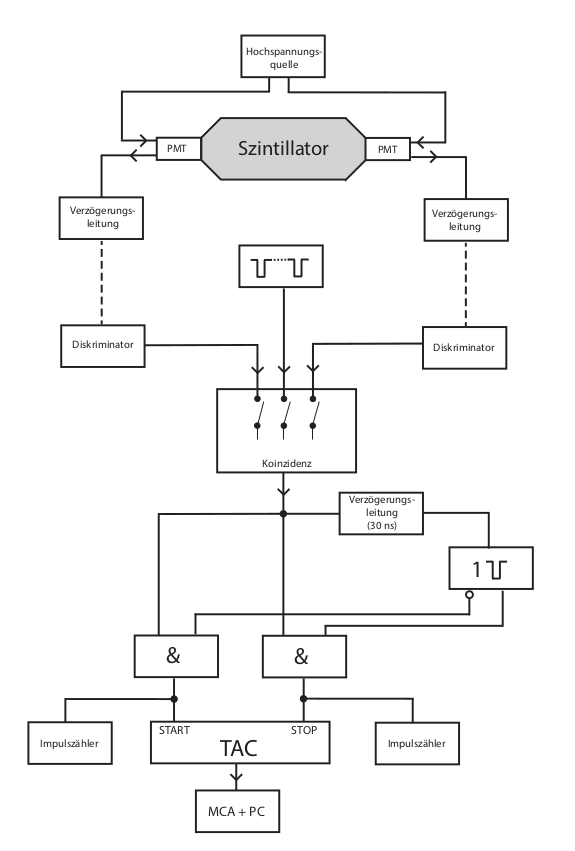
\includegraphics[width=0.8\textwidth]{./Bilder/aufbau.png}
	\caption{Blockschaltbild des Versuchsaufbaus}\label{fig:aufbau}
\end{figure}

In Abbildung \ref{fig:aufbau} ist der Aufbau abgebildet.
Der Szintillator Tank mit den zwei PMT Detektoren ist über zwei Verzögerungsleitungnen
und zwei Diskriminatoren an eine Koinzidenzschaltung angeschlossen. 
Die Diskriminatoren filtern die Signale nach der Stärke, die Koinzidenzschaltung
lässt die Signale nur durch wenn sie von beiden PMT gleichzeitig kommt.
Signale die von den PMT gleichzeitig kommen sind durch ein geladenes Teilchen im Szintillator
ausgelöst, das beide Detektoren gleichzeitig aktivieren kann und nicht durch eine zufällige 
thermische Kaskade in einem der PMT.

Der zweite Teil der Schaltung ist dazu da die Signale von den Myonen herauszufiltern, die tatsächlich
in der Myonenkammer zerfallen


%% Monoflop Zeug Signal Kommm